\documentclass{article}
\usepackage{amsmath}
\usepackage{amssymb}
\usepackage{graphicx}
\usepackage{hyperref}
\usepackage[version=4]{mhchem}


\begin{document}
\section*{Problem}
In the adjoining figure \(A M\) and \(B N\) are parallel to each other and are tangent to the circle \(O\), with \(A\) and \(B\) the points of tangency. \(M P N\) is a third tangent with \(P\) as point of tangency. Show that the radius of the circle is \(r=\sqrt{A M \times B N}\).\\
\centering
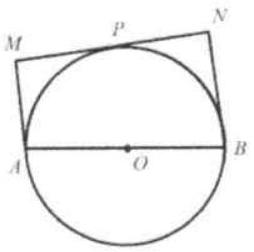
\includegraphics[width=\textwidth]{images/155(1).jpg}

\section*{Solution}
Connect OM, OP, ON .\\
Since \(A\) and \(P\) are two tangent points, \(A M=P M\).\\
\(O A=O P=r . O M=O M\).\\
So \(\triangle A O M \cong \triangle P O M\). Then \(\angle A O M=\angle P O M=\alpha\).

Similarly, \(\angle P O N=\angle B O N=\beta\).\\
\centering
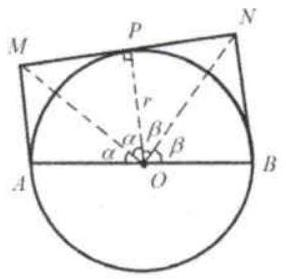
\includegraphics[width=\textwidth]{images/158(1).jpg}

Since \(2 \alpha+2 \beta=180^{\circ}, \alpha+\beta=\angle M O N=90^{\circ}\),\\
Thus \(P O^{2}=M P \times P N=A M \times B N\), or\\
\(r^{2}=A M \times B N \quad \Rightarrow \quad r=\sqrt{A M \times B N}\)

\end{document}
